\documentclass{if-beamer}
\usepackage[english]{babel}
\usepackage[absolute,overlay]{textpos}
\usepackage{booktabs}
\usepackage{tikz}
\usetikzlibrary{arrows.meta, positioning, fit, backgrounds, calc}

% Single logo: IIT Mandi only
\logoleft{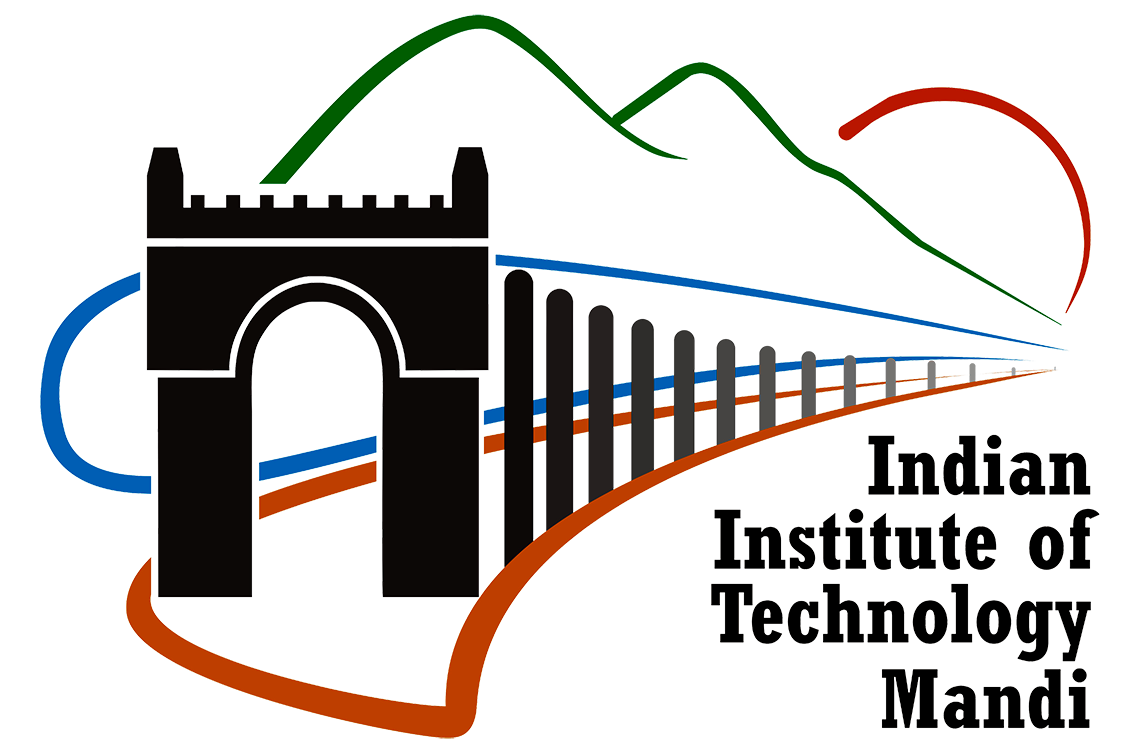
\includegraphics[width=4cm]{iitlogo.png}}

% --------------------------------------------------- %
%                  Presentation info                  %
% --------------------------------------------------- %
\title[Final Presentation]{\Huge\textbf{AR525: Reinforcement Learning in Robotics}}
\subtitle{\Large{Final Presentation --- MC-PILOT: Reproduction, Analysis \& Extension}}

\author[]{
    \large \textbf{Group-3} \\[0.5em]
    \small Rishang Yadav, Bhumika Gupta, Aarya Agarwal, Yajesh Chandra\newline\newline
}

\institute[IIT Mandi]{}

\subject{Pick \& Throw Operations using RL}

% --------------------------------------------------- %
%                    Title + Outline                  %
% --------------------------------------------------- %

\begin{document}

\begin{frame}
  \titlepage
\end{frame}

\begin{frame}{Outline}
  \tableofcontents
\end{frame}

% --------------------------------------------------- %
%                    Presentation                     %
% --------------------------------------------------- %

%%%%%%%%%%%%%%%%%%%%%%%%%%%%%%%%%%%%%%%%%%%%%%%%%%%%%%%%%%%%%
\section{Problem \& Motivation}

\begin{frame}{Pick-and-Throw Operations}
    \begin{columns}[T]
        \begin{column}{0.52\textwidth}
            \textbf{The Task}
            \begin{itemize}
                \item Robot arm grasps a ball and \textbf{throws} it into a target bin at distance $0.75$--$2.4$\,m
                \item Ball follows a parabolic + drag trajectory after release --- physics is \textit{known but noisy}
                \item Gap between \textbf{commanded} and \textbf{delivered} velocity is random and arm-dependent
                \item Naive approach (model-free RL): needs \textbf{100s--1000s} of real throws
            \end{itemize}
        \end{column}
        \begin{column}{0.44\textwidth}
            \begin{block}{Key Question}
                \centering
                \textit{Can a robot learn to throw accurately from just $\mathbf{\sim}$\textbf{10 attempts?}}
            \end{block}
            \vspace{0.5em}
            \textbf{Why it's hard}
            \begin{itemize}
                \item Precise gripper timing at high speed
                \item Object mass \& drag uncertainty
                \item Physical wear limits real trials
            \end{itemize}
        \end{column}
    \end{columns}
\end{frame}

%%%%%%%%%%%%%%%%%%%%%%%%%%%%%%%%%%%%%%%%%%%%%%%%%%%%%%%%%%%%%
\section{Background: MC-PILOT}

\begin{frame}{Algorithmic Lineage}
    \begin{center}
    \small
    \begin{tabular}{llll}
        \toprule
        \textbf{Algorithm} & \textbf{Year} & \textbf{Key Idea} & \textbf{Data Needed} \\
        \midrule
        Model-free RL (DQN, PPO) & 2013--20 & Learn from reward only & $\sim$1000s trials \\
        PILCO & 2011 & GP dynamics + analytic gradient & $\sim$50 trials \\
        MC-PILCO & 2022 & Monte Carlo gradient through GP & $\sim$20--50 trials \\
        \textbf{MC-PILOT} & \textbf{2025} & Single-shot throwing adaptation & $\mathbf{\sim}$\textbf{5+10 throws} \\
        \bottomrule
    \end{tabular}
    \end{center}
    \vspace{0.5em}
    \textbf{Why Gaussian Processes for dynamics?}
    \begin{itemize}
        \item Exact uncertainty quantification --- policy gradient knows \textit{model confidence}
        \item Bayesian: posterior updates analytically with each new throw
        \item Data-efficient --- 5 exploration throws suffice to bootstrap learning
    \end{itemize}
\end{frame}

\begin{frame}{MC-PILOT: Two Key Modifications over MC-PILCO}
    \begin{block}{Modification 1 --- Single-Shot Policy}
        \begin{itemize}
            \item Standard MC-PILCO fires the policy at \textit{every} timestep (suitable for balancing tasks)
            \item Throwing: policy fires \textbf{once} $\rightarrow$ choose release speed $\rightarrow$ ball is in free flight
            \item Policy: $\pi_\theta(P) \rightarrow v$ \quad State: $\tilde{x} = [x,y,z,v_x,v_y,v_z,P_x,P_y] \in \mathbb{R}^8$
        \end{itemize}
    \end{block}
    \begin{block}{Modification 2 --- Gripper Delay Estimation}
        \begin{itemize}
            \item Real gripper doesn't open instantly $\Rightarrow$ random delay $\Rightarrow$ velocity undershoot
            \item MC-PILOT fits delay distribution $t_d \sim \mathcal{U}(a,b)$ via Bayesian Optimisation on hardware
            \item Enables deployment on \textbf{real hardware} (Franka Panda + real bin)
        \end{itemize}
    \end{block}
    \begin{alertblock}{Paper Claim (Verified)}
        $\sim$10 learning throws $\rightarrow$ near-100\% hit rate. Model-free baselines need $100\times$ more data.
    \end{alertblock}
\end{frame}

%%%%%%%%%%%%%%%%%%%%%%%%%%%%%%%%%%%%%%%%%%%%%%%%%%%%%%%%%%%%%
\section{Our Contributions}

\begin{frame}{What We Set Out To Do}
    We replaced Gazebo/ROS with a \textbf{pure Python + PyBullet} environment (no ROS required for ball physics).

    \vspace{0.5em}
    \begin{center}
    \small
    \begin{tabular}{ll}
        \toprule
        \textbf{Goal} & \textbf{Status} \\
        \midrule
        Reproduce MC-PILOT baseline ($z=0.5$\,m, Franka Panda) & \textcolor{green!60!black}{$\checkmark$ Done} \\
        Diagnose \& fix silent implementation bugs & \textcolor{green!60!black}{$\checkmark$ Done} \\
        Generalise to elevated release heights ($z=1.0,1.5,2.0$\,m) & \textcolor{green!60!black}{$\checkmark$ Done} \\
        Generalise to 3 different robot arms & \textcolor{green!60!black}{$\checkmark$ Done} \\
        Model arm-side noise (slip, jitter, salt-pepper) & \textcolor{green!60!black}{$\checkmark$ Done} \\
        Wind conditions (constant, gusts, turbulence) & \textcolor{green!60!black}{$\checkmark$ Done} \\
        OpenCV + YOLO bin detection $\rightarrow$ autonomous targeting & \textcolor{green!60!black}{$\checkmark$ Done} \\
        \bottomrule
    \end{tabular}
    \end{center}
\end{frame}

\begin{frame}{Why PyBullet for RL Training?}
    \centering
    \small
    \begin{tabular}{p{2.3cm}p{4.3cm}p{3.8cm}}
        \toprule
        \textbf{Aspect} & \textbf{PyBullet Advantage} & \textbf{Gazebo Limitation} \\
        \midrule
        Sample efficiency & High rollout throughput (fast step + reset) & Lower throughput due to overhead \\
        Policy learning & Better exploration of release timing \& velocity & Fewer episodes $\rightarrow$ slower convergence \\
        Training loop & Tight Python RL loop integration & ROS-based loop adds latency \\
        Episode reset & Fast environment reinitialization & Slower world reset/reload \\
        \bottomrule
    \end{tabular}
\end{frame}

%%%%%%%%%%%%%%%%%%%%%%%%%%%%%%%%%%%%%%%%%%%%%%%%%%%%%%%%%%%%%
\section{Two Convergence Rules}

\begin{frame}{Rule 1 --- Stratified Exploration}
    \begin{block}{The Problem with Random Exploration}
        \begin{itemize}
            \item Random exploration with 5 throws can accidentally draw 4 \textit{low-speed} throws
            \item \textbf{Config B, seed=1, $z=1.0$\,m}: GP has no data on high-speed dynamics $\Rightarrow$ \textbf{0/10 hits}
        \end{itemize}
    \end{block}
    \begin{block}{Fix: Stratified Band Sampling}
        Divide $[0, u_M]$ into $N_\text{exp}$ equal bands; sample exactly one throw per band:
        \[
            v_i \sim \mathcal{U}\!\left(\frac{(i-1)\,u_M}{N_\text{exp}},\ \frac{i\,u_M}{N_\text{exp}}\right),\quad i = 1,\ldots,N_\text{exp}
        \]
        Guarantees full speed-range coverage regardless of random seed. Zero extra hardware trials.
    \end{block}
    \begin{exampleblock}{Evidence}
        Config B-random seed=1 $\rightarrow$ \textbf{0/10}. \quad Same config, stratified $\rightarrow$ \textbf{10/10}.
    \end{exampleblock}
\end{frame}

\begin{frame}{Rule 2 --- RBF Lengthscale Must Match Target Range}
    \begin{block}{RBF Sensitivity Formula}
        \[
            S(d, \ell_s) = \exp\!\left(-\frac{d^2}{2\ell_s^2}\right)
        \]
        $S \to 1$: policy outputs \textit{identical} speed for all targets.\quad $S \to 0$: targets are well discriminated.
    \end{block}

    Paper uses $\ell_s = 1.0$\,m everywhere. For \textbf{Config E} (in elevated target range $0.35$\,m):
    \[
        S = \exp\!\left(-\frac{0.35^2}{2 \times 1.0^2}\right) = 0.941 \quad \Rightarrow \text{policy is \textbf{constant} for all targets}
    \]

    \begin{block}{Scaling Rule}
        \[
            \ell_s^* \approx 0.15 \times \Delta_\text{range}
        \]
        This maintains $S \approx 0.066$ --- the same discriminability level as the working configs.
    \end{block}
    \begin{exampleblock}{Evidence}
        Config E failed \textbf{4 consecutive iterations} with $\ell_s = 1.0$\,m.
        Changed to $\ell_s = 0.15$\,m $\rightarrow$ \textbf{10/10 hits immediately}.
    \end{exampleblock}
\end{frame}



%%%%%%%%%%%%%%%%%%%%%%%%%%%%%%%%%%%%%%%%%%%%%%%%%%%%%%%%%%%%%
\section{Study 1: Baseline \& Elevated Heights}

\begin{frame}{Baseline Result: 5/5 Hits in 10 Total Throws}
    \begin{columns}[T]
        \begin{column}{0.45\textwidth}
            \small
            \begin{tabular}{cccc}
                \toprule
                \textbf{Throw} & \textbf{Phase} & \textbf{Error} & \textbf{Hit?} \\
                \midrule
                1--5 & Exploration & 0.02--1.09\,m & --- \\
                6 & Trial 1 & 8.5\,cm & \textcolor{green!60!black}{$\checkmark$} \\
                7 & Trial 2 & 3.3\,cm & \textcolor{green!60!black}{$\checkmark$} \\
                8 & Trial 3 & 2.3\,cm & \textcolor{green!60!black}{$\checkmark$} \\
                9 & Trial 4 & 1.7\,cm & \textcolor{green!60!black}{$\checkmark$} \\
                10 & Trial 5 & 0.8\,cm & \textcolor{green!60!black}{$\checkmark$} \\
                \bottomrule
            \end{tabular}
            \vspace{0.5em}

            \textbf{Cost trajectory:}\\
            $0.74 \xrightarrow{\text{Trial 1}} 0.009 \xrightarrow{\text{Trial 5}} 0.001$
        \end{column}
        \begin{column}{0.52\textwidth}
            \begin{block}{Physical Meaning}
                GP learns the speed-to-range curve from \textbf{5 random throws}. Policy optimisation (1500 gradient steps/trial) finds the exact release speed per target. By trial 5, errors are \textbf{sub-centimetre}.
            \end{block}
            \vspace{0.3em}
            \textit{Config A: $z_\text{rel} = 0.5$\,m, $\ell_M = 1.75$\,m, Franka Panda, no noise.}
        \end{column}
    \end{columns}
\end{frame}

\begin{frame}{Generalising to Elevated Release Heights}
    \textbf{Engineering challenges:}
    \begin{itemize}
        \item KUKA iiwa7 joint limits cap EE speed at $\sim$2.5\,m/s; throw needs 3.5\,m/s $\rightarrow$ \textit{decoupled}: ball velocity set via \texttt{resetBaseVelocity}, arm is cosmetic
        \item EE cannot reach $z=1.5$\,m from ground $\rightarrow$ mount arm on pedestal: $z_\text{base} = z_\text{rel} - 0.5$\,m
    \end{itemize}
    \vspace{0.5em}
    \begin{center}
    \scriptsize
    \begin{tabular}{llllll}
        \toprule
        \textbf{Config} & \textbf{$z_\text{rel}$} & \textbf{Exploration} & \textbf{Hit rate} & \textbf{Mean error} & \textbf{Cost trajectory} \\
        \midrule
        A        & 0.5\,m & Random & 100\% (5/5) & 33\,mm & $0.740 \rightarrow 0.001$ \\
        B        & 1.0\,m & Random & 100\% (10/10) & 20\,mm & $0.882 \rightarrow 0.005$ \\
        B-Strat  & 1.0\,m & Stratified & 100\% (10/10) & 20\,mm & $0.811 \rightarrow 0.003$ \\
        C-Strat  & 1.5\,m & Stratified & 100\% (10/10) & 14\,mm & $0.809 \rightarrow 0.085$ \\
        D-Strat  & 2.0\,m & Stratified & 100\% (10/10) & 16\,mm & $0.827 \rightarrow 0.024$ \\
        E-Strat5 & 0\,m & Stratified, $\ell_s=0.15$ & 80\% (12/15) & 69\,mm$^\dagger$ & $--- \rightarrow 0.031$ \\
        \bottomrule
    \end{tabular}
    \end{center}
    \vspace{0.3em}
    \textit{$^\dagger$ E-Strat5: first 5 throws still converging (mean 155\,mm); throws 6--15 post-convergence achieved 100\% hit rate with mean error 26\,mm. Config A early-stopped at step 1204 on Trial 5; trial errors: 85 $\rightarrow$ 33 $\rightarrow$ 23 $\rightarrow$ 17 $\rightarrow$ 8\,mm.}
\end{frame}

%%%%%%%%%%%%%%%%%%%%%%%%%%%%%%%%%%%%%%%%%%%%%%%%%%%%%%%%%%%%%
\section{Study 2: Multi-Arm Generalisation}

\begin{frame}{Three Robot Arms: Franka Panda, KUKA iiwa7, xArm6}
    \begin{columns}[T]
        \begin{column}{0.48\textwidth}
            \begin{block}{Key Architectural Insight --- Decoupled Design}
                \begin{itemize}
                    \item RL trains on \textbf{ball physics only} (NumPy ballistic simulator)
                    \item Joint velocities calculated depending on the arm to set ball velocity at release.
                    \item Joint tracking error is substituted by our own error; matching MC-PILOT.
                \end{itemize}
            \end{block}
        \end{column}
        \begin{column}{0.48\textwidth}
            \centering
            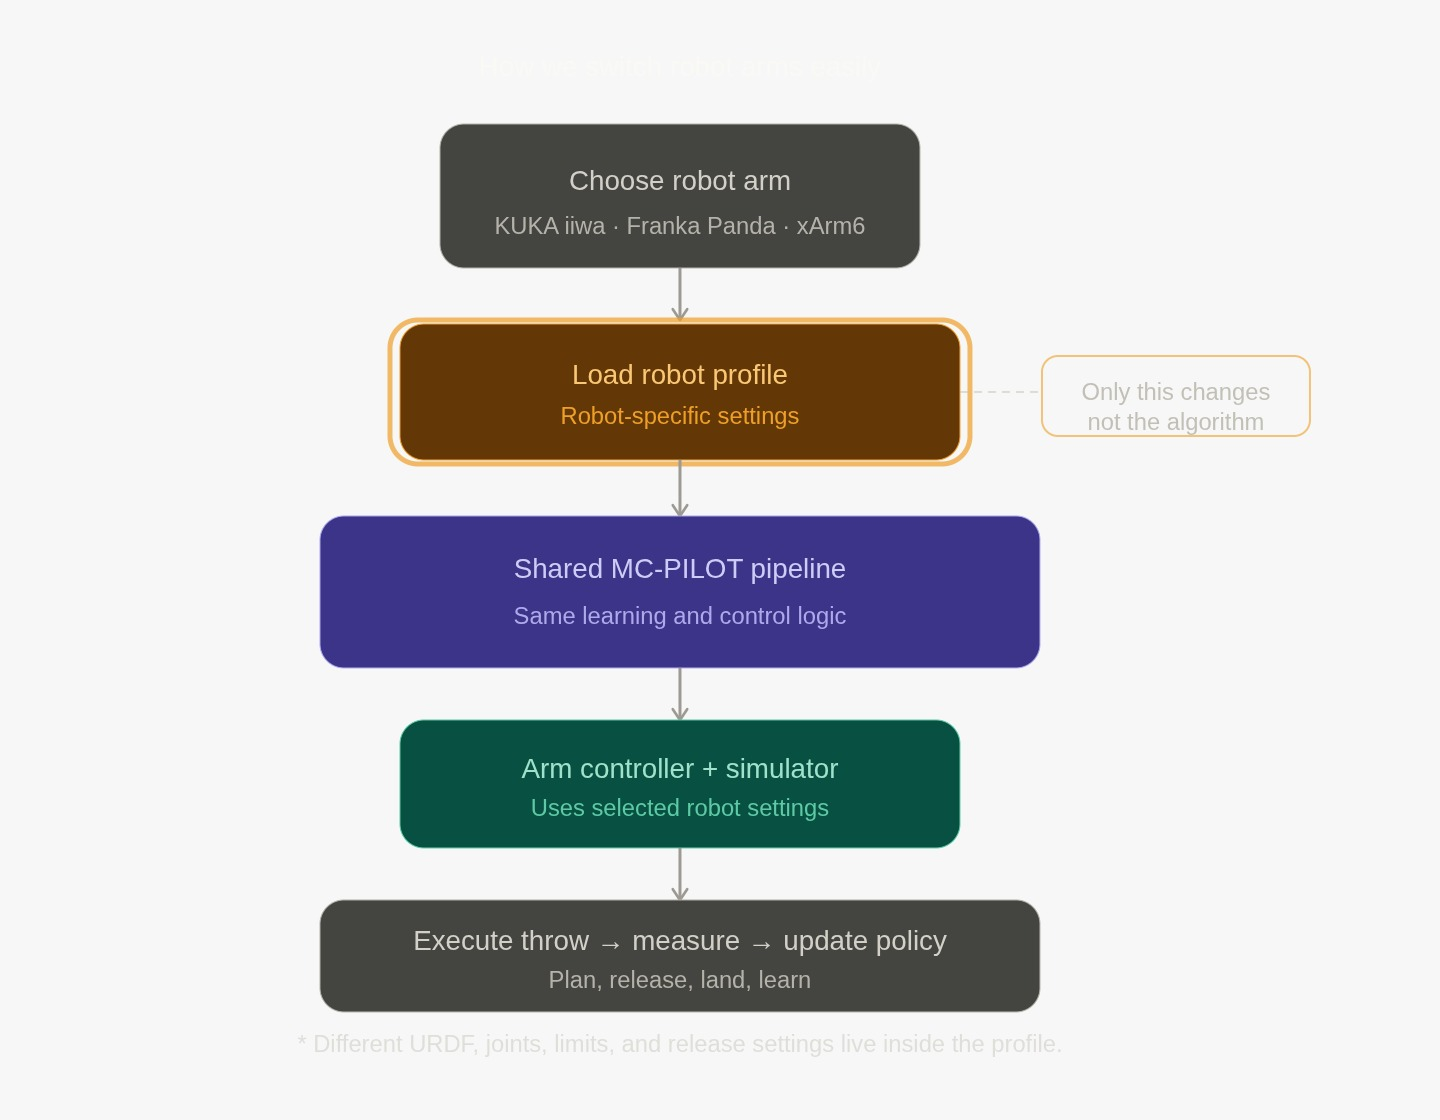
\includegraphics[width=\textwidth,height=0.7\textheight,keepaspectratio]{robot_arm_flowchart.jpeg}
        \end{column}
    \end{columns}
\end{frame}

\begin{frame}{Cross-Arm Results}
    \centering
    \includegraphics[width=0.94\textwidth,height=0.78\textheight,keepaspectratio]{cross-arm-results.png}
\end{frame}

%%%%%%%%%%%%%%%%%%%%%%%%%%%%%%%%%%%%%%%%%%%%%%%%%%%%%%%%%%%%%
\section{Study 3: Noise Models}

\begin{frame}{Arm-Side Stochasticity: Making RL Non-Trivial}
    \begin{columns}[T]
        \begin{column}{0.48\textwidth}
            \textbf{Why noise matters}
            \begin{itemize}
                \item Without noise: a ballistic inverter solves the task in one step --- \textbf{RL adds no value}
                \item With noise: policy must learn to compensate --- \textbf{RL is necessary}
            \end{itemize}
            \vspace{0.5em}
            \textbf{Two learnable noise types:}
            \begin{itemize}
                \item \textit{VelocitySlipNoise:} $v_\text{actual} = (1-\alpha)\,v_\text{cmd} + \mathcal{N}(0,\sigma^2)$\\
                Systematic undershoot; policy must learn to command $v/(1-\alpha)$
                \item \textit{Salt-and-Pepper:} velocity component randomly replaced by a spike; models encoder glitches
            \end{itemize}
        \end{column}
        \begin{column}{0.48\textwidth}
            \begin{alertblock}{Key Theorem (Proven)}
                Zero-mean \textbf{symmetric} noise does \textbf{not} shift the optimal policy:
                \[
                    \nabla_{v^*} J_\text{aware} = \nabla_{v^*} J_\text{naive}
                \]
                Only \textbf{biased} noise (slip, jitter) is learnable and compensable.
                Paper's gripper delay model is biased --- which is why it works on hardware.
            \end{alertblock}
        \end{column}
    \end{columns}
\end{frame}

\begin{frame}[plain]{Noise Results: Aware Policy vs.\ Naive Policy}
    \centering
    \vspace*{-0.2cm}
    \makebox[\paperwidth][c]{%
        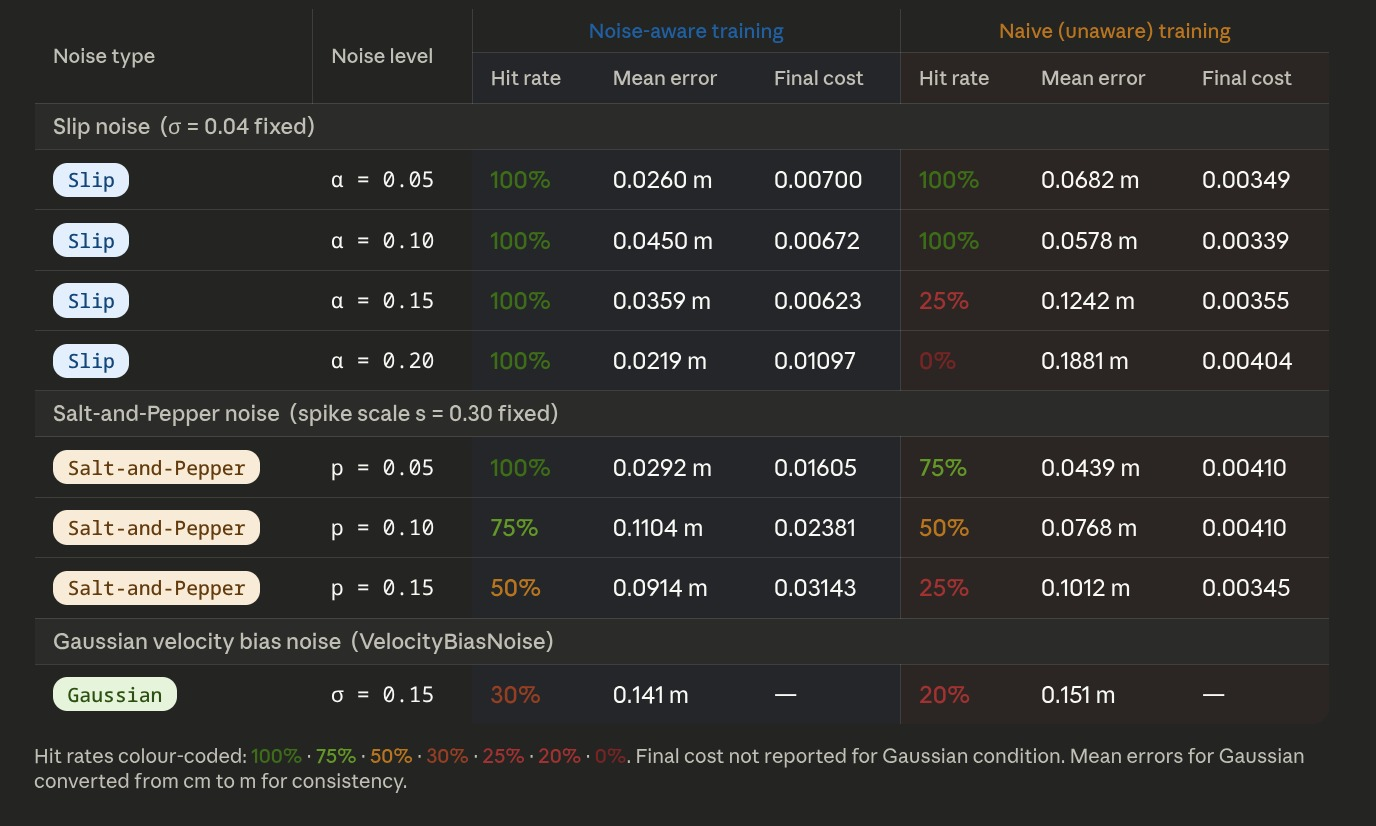
\includegraphics[width=0.88\paperwidth,height=0.88\paperheight,keepaspectratio]{noise_results.jpeg}%
    }
\end{frame}

%%%%%%%%%%%%%%%%%%%%%%%%%%%%%%%%%%%%%%%%%%%%%%%%%%%%%%%%%%%%%
\section{Study 4: Wind Robustness}

\begin{frame}{Wind Modelling \& Environmental Disturbances}
    \begin{alertblock}{Problem Context}
        \begin{itemize}
            \item The standard MC-PILOT model assumes \textbf{calm, still air}, limiting reliability in semi-outdoor deployments where modest wind can shift lightweight payloads.
        \end{itemize}
    \end{alertblock}
    \begin{block}{Experimental Setup}
        \begin{itemize}
            \item Extended the physics simulator with a \textbf{wind force term} integrated into the aerodynamic drag equation.
            \item Evaluated against three dynamic wind conditions: \textbf{constant wind}, \textbf{random gusts} (step changes in $\mathbf{w}$), and \textbf{turbulence} (Gaussian noise on $\mathbf{w}$).
            \item Compared a standard \textbf{Wind-Blind} model (8D state) against a \textbf{Wind-Aware} model (10D state with explicit wind input) to determine if the GP implicitly absorbs disturbances.
        \end{itemize}
    \end{block}
\end{frame}

\begin{frame}{Empirical Findings: Wind-Aware vs. Wind-Blind}
    \begin{block}{Key Results}
        \begin{itemize}
            \item \textbf{Accuracy Degradation:} Constant wind degrades base performance (Hit rate dropped from 73\% to 47\% under strong wind).
            \item \textbf{Implicit Absorption:} Surprisingly, the \textbf{Wind-Blind (8D)} model consistently \textbf{outperformed} the Wind-Aware (10D) model across all dynamic conditions.
            \item For example, in Turbulence (W3), the blind baseline achieved a 60\% hit rate compared to the aware model's 47\%.
        \end{itemize}
    \end{block}
    \begin{alertblock}{Conclusion}
        Expanding the state space to 10D increased the learning complexity beyond what the GP could efficiently sample within limited trials. The 8D model was robust enough to implicitly absorb the wind disturbances as a bias term.
    \end{alertblock}
\end{frame}

\begin{frame}{Performance Analysis: Hit Rates}
    \begin{figure}
        \centering
        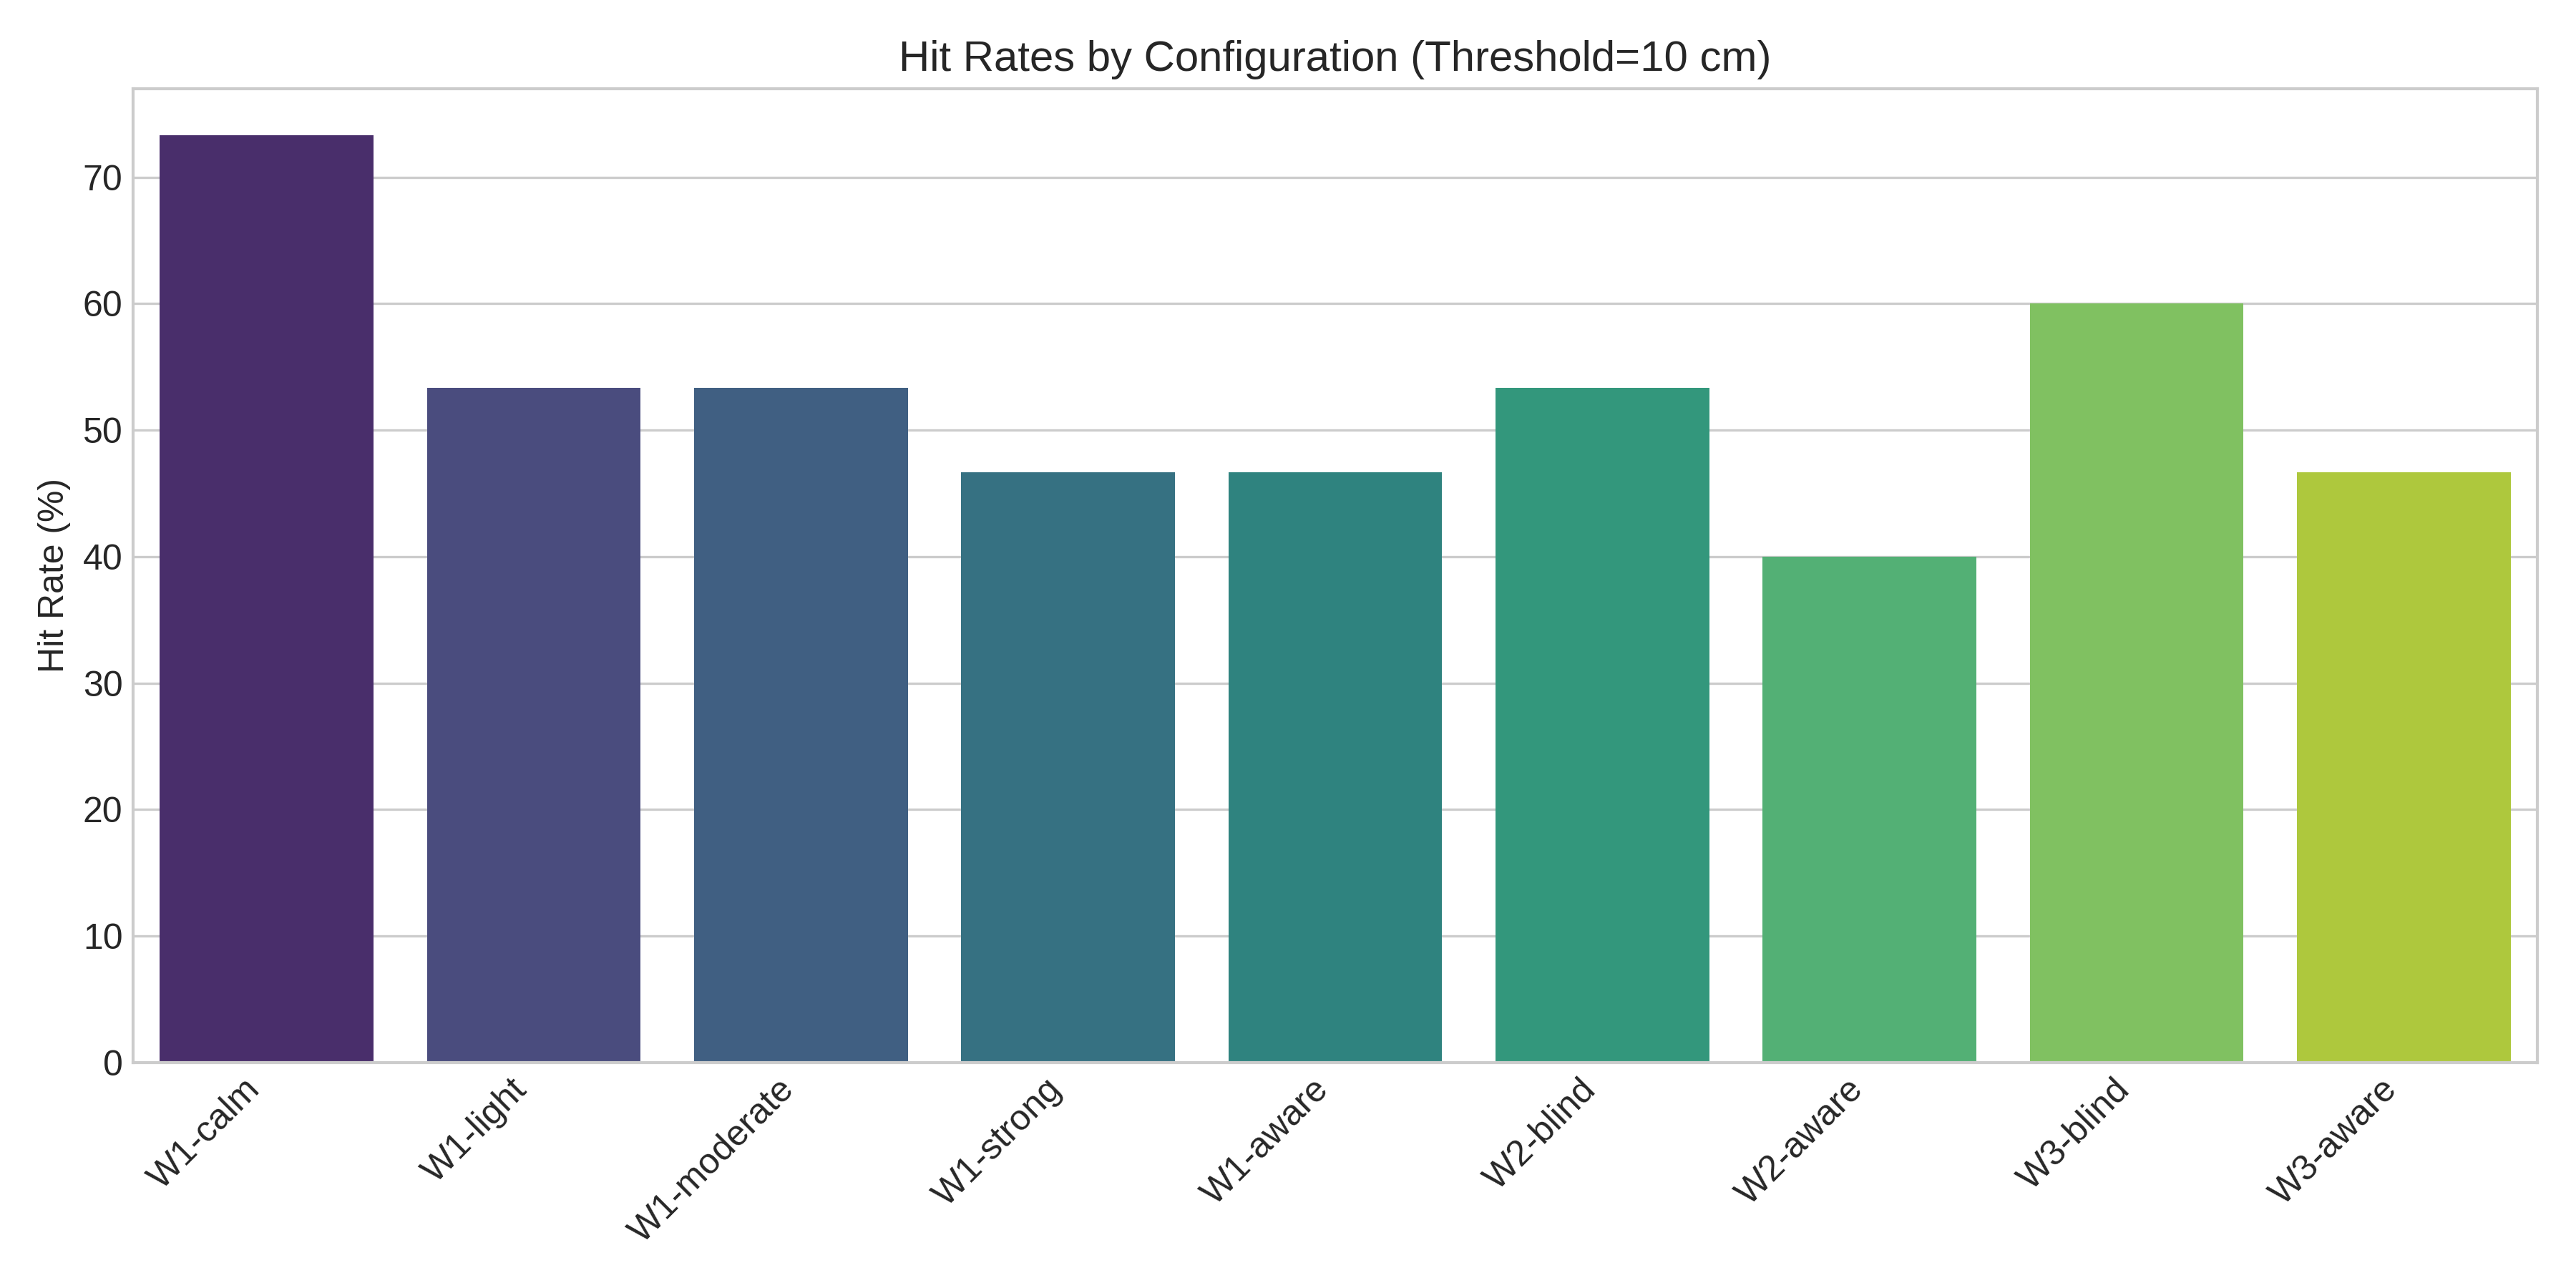
\includegraphics[width=0.85\textwidth]{performance_analysis_plots/hit_rates.png}
        \caption{Comparison of Hit Rates (landing within 10cm threshold) across configurations.}
    \end{figure}
\end{frame}

\begin{frame}{Performance Analysis: Error Variance}
    \begin{figure}
        \centering
        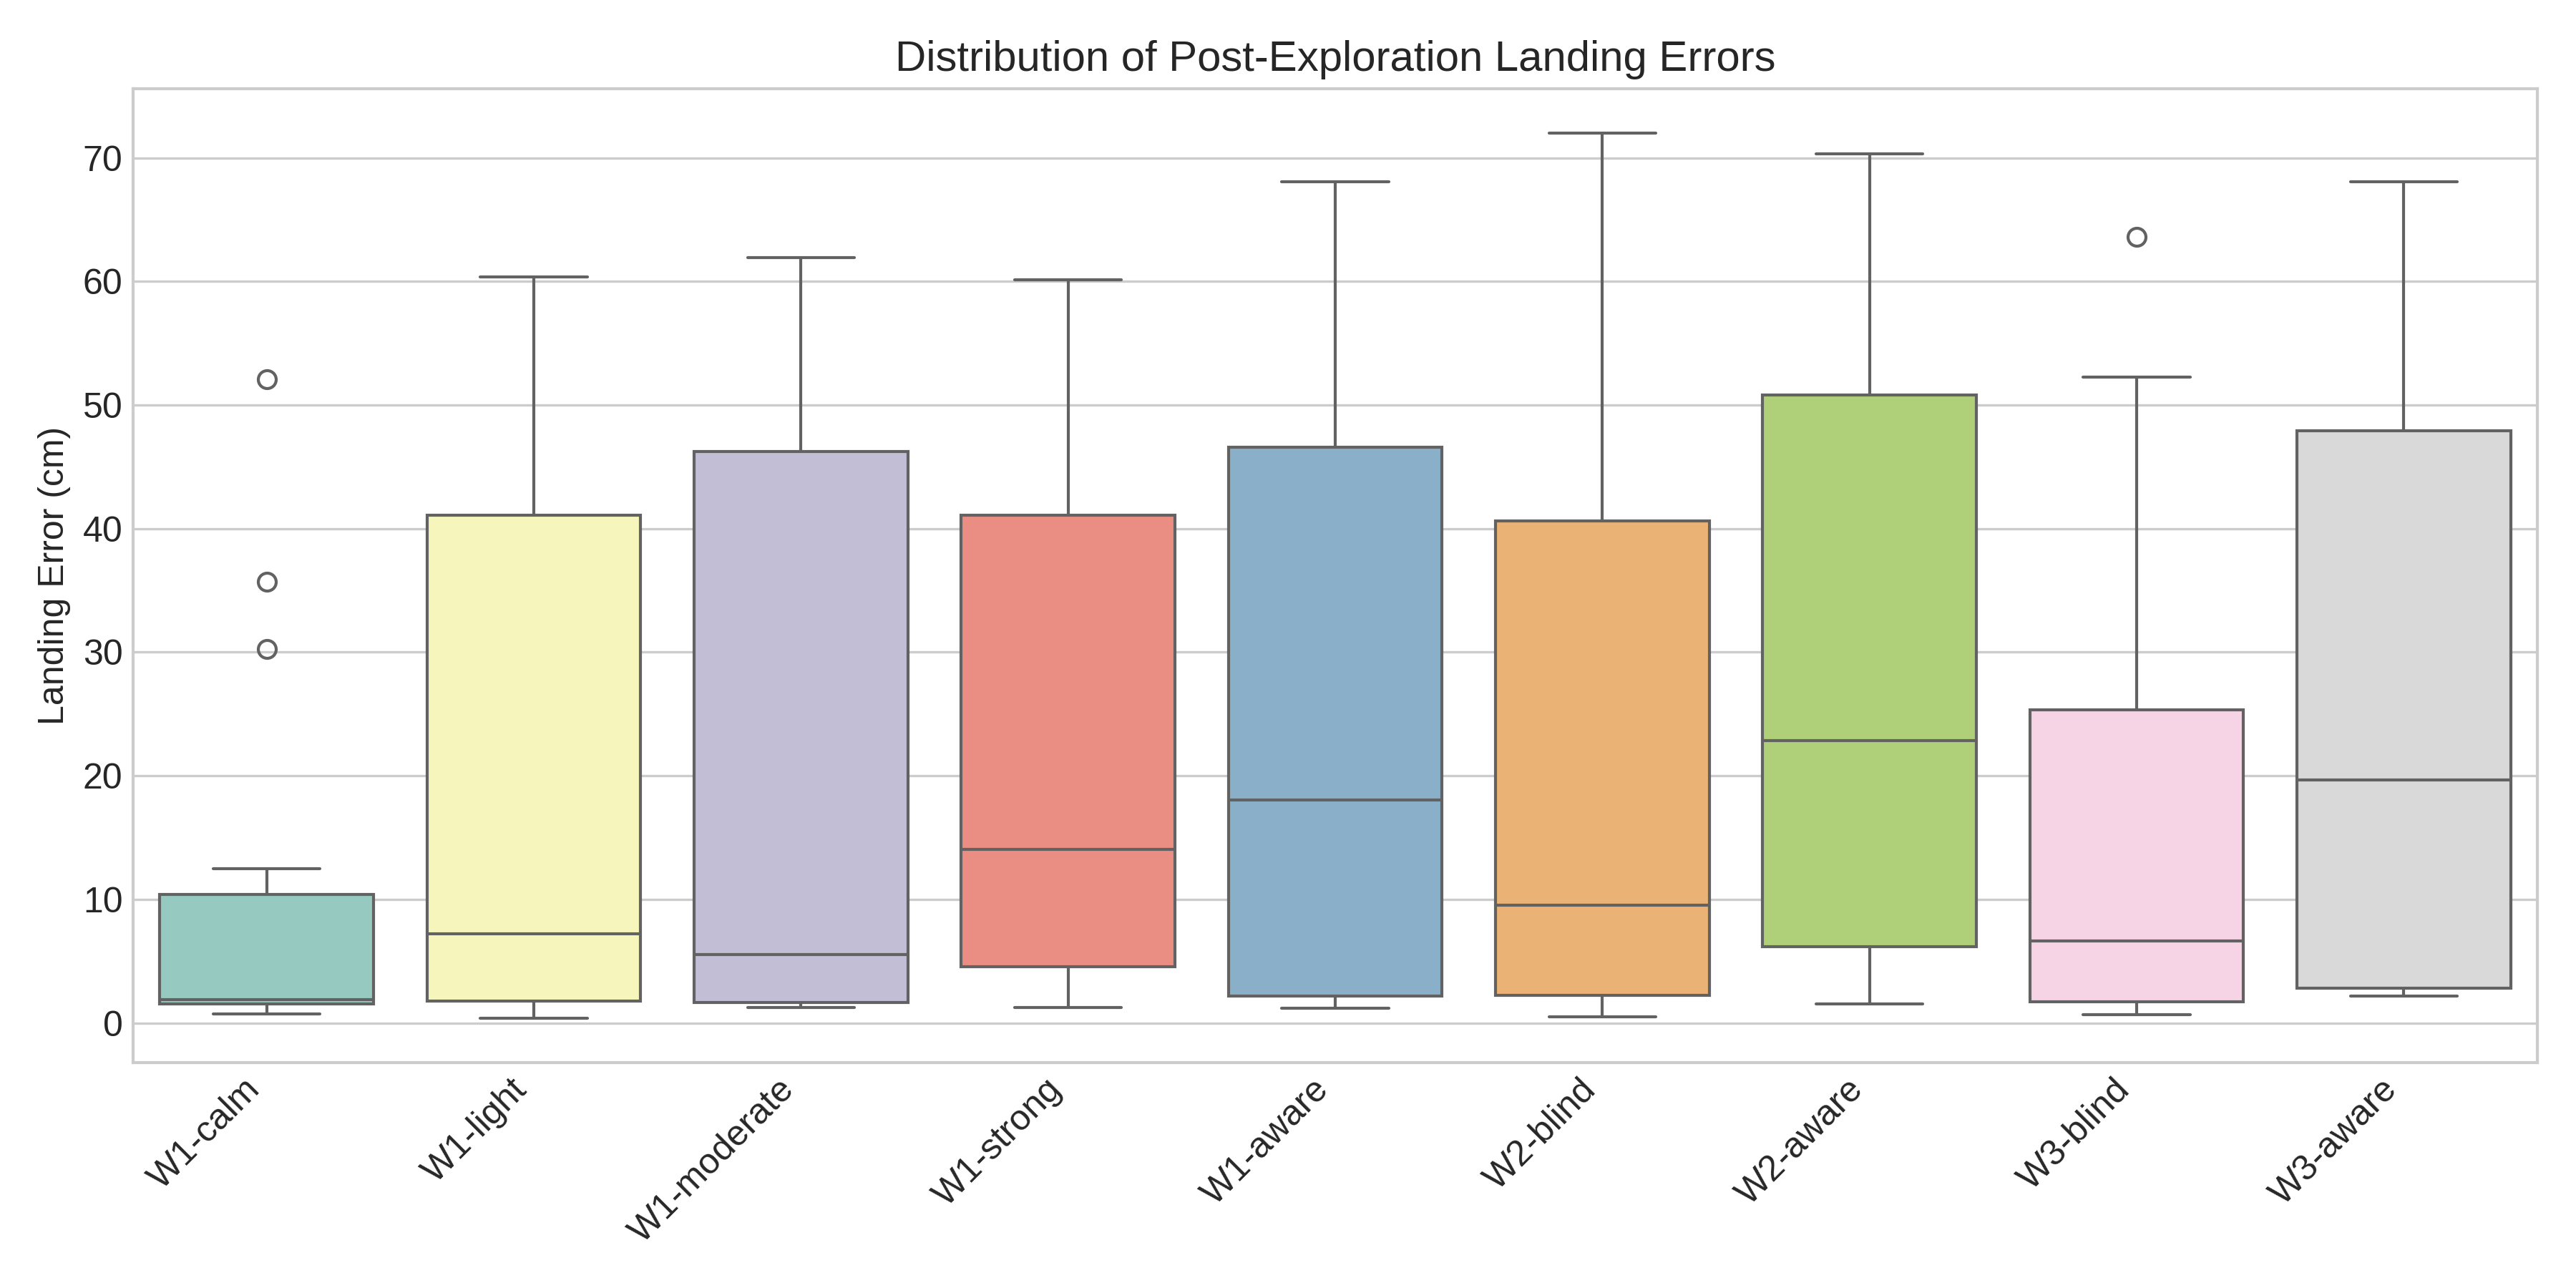
\includegraphics[width=0.85\textwidth]{performance_analysis_plots/error_distributions_boxplot.png}
        \caption{Landing Error Variance and Distribution for post-exploration trials.}
    \end{figure}
\end{frame}

\begin{frame}{Performance Analysis: Learning Convergence}
    \begin{figure}
        \centering
        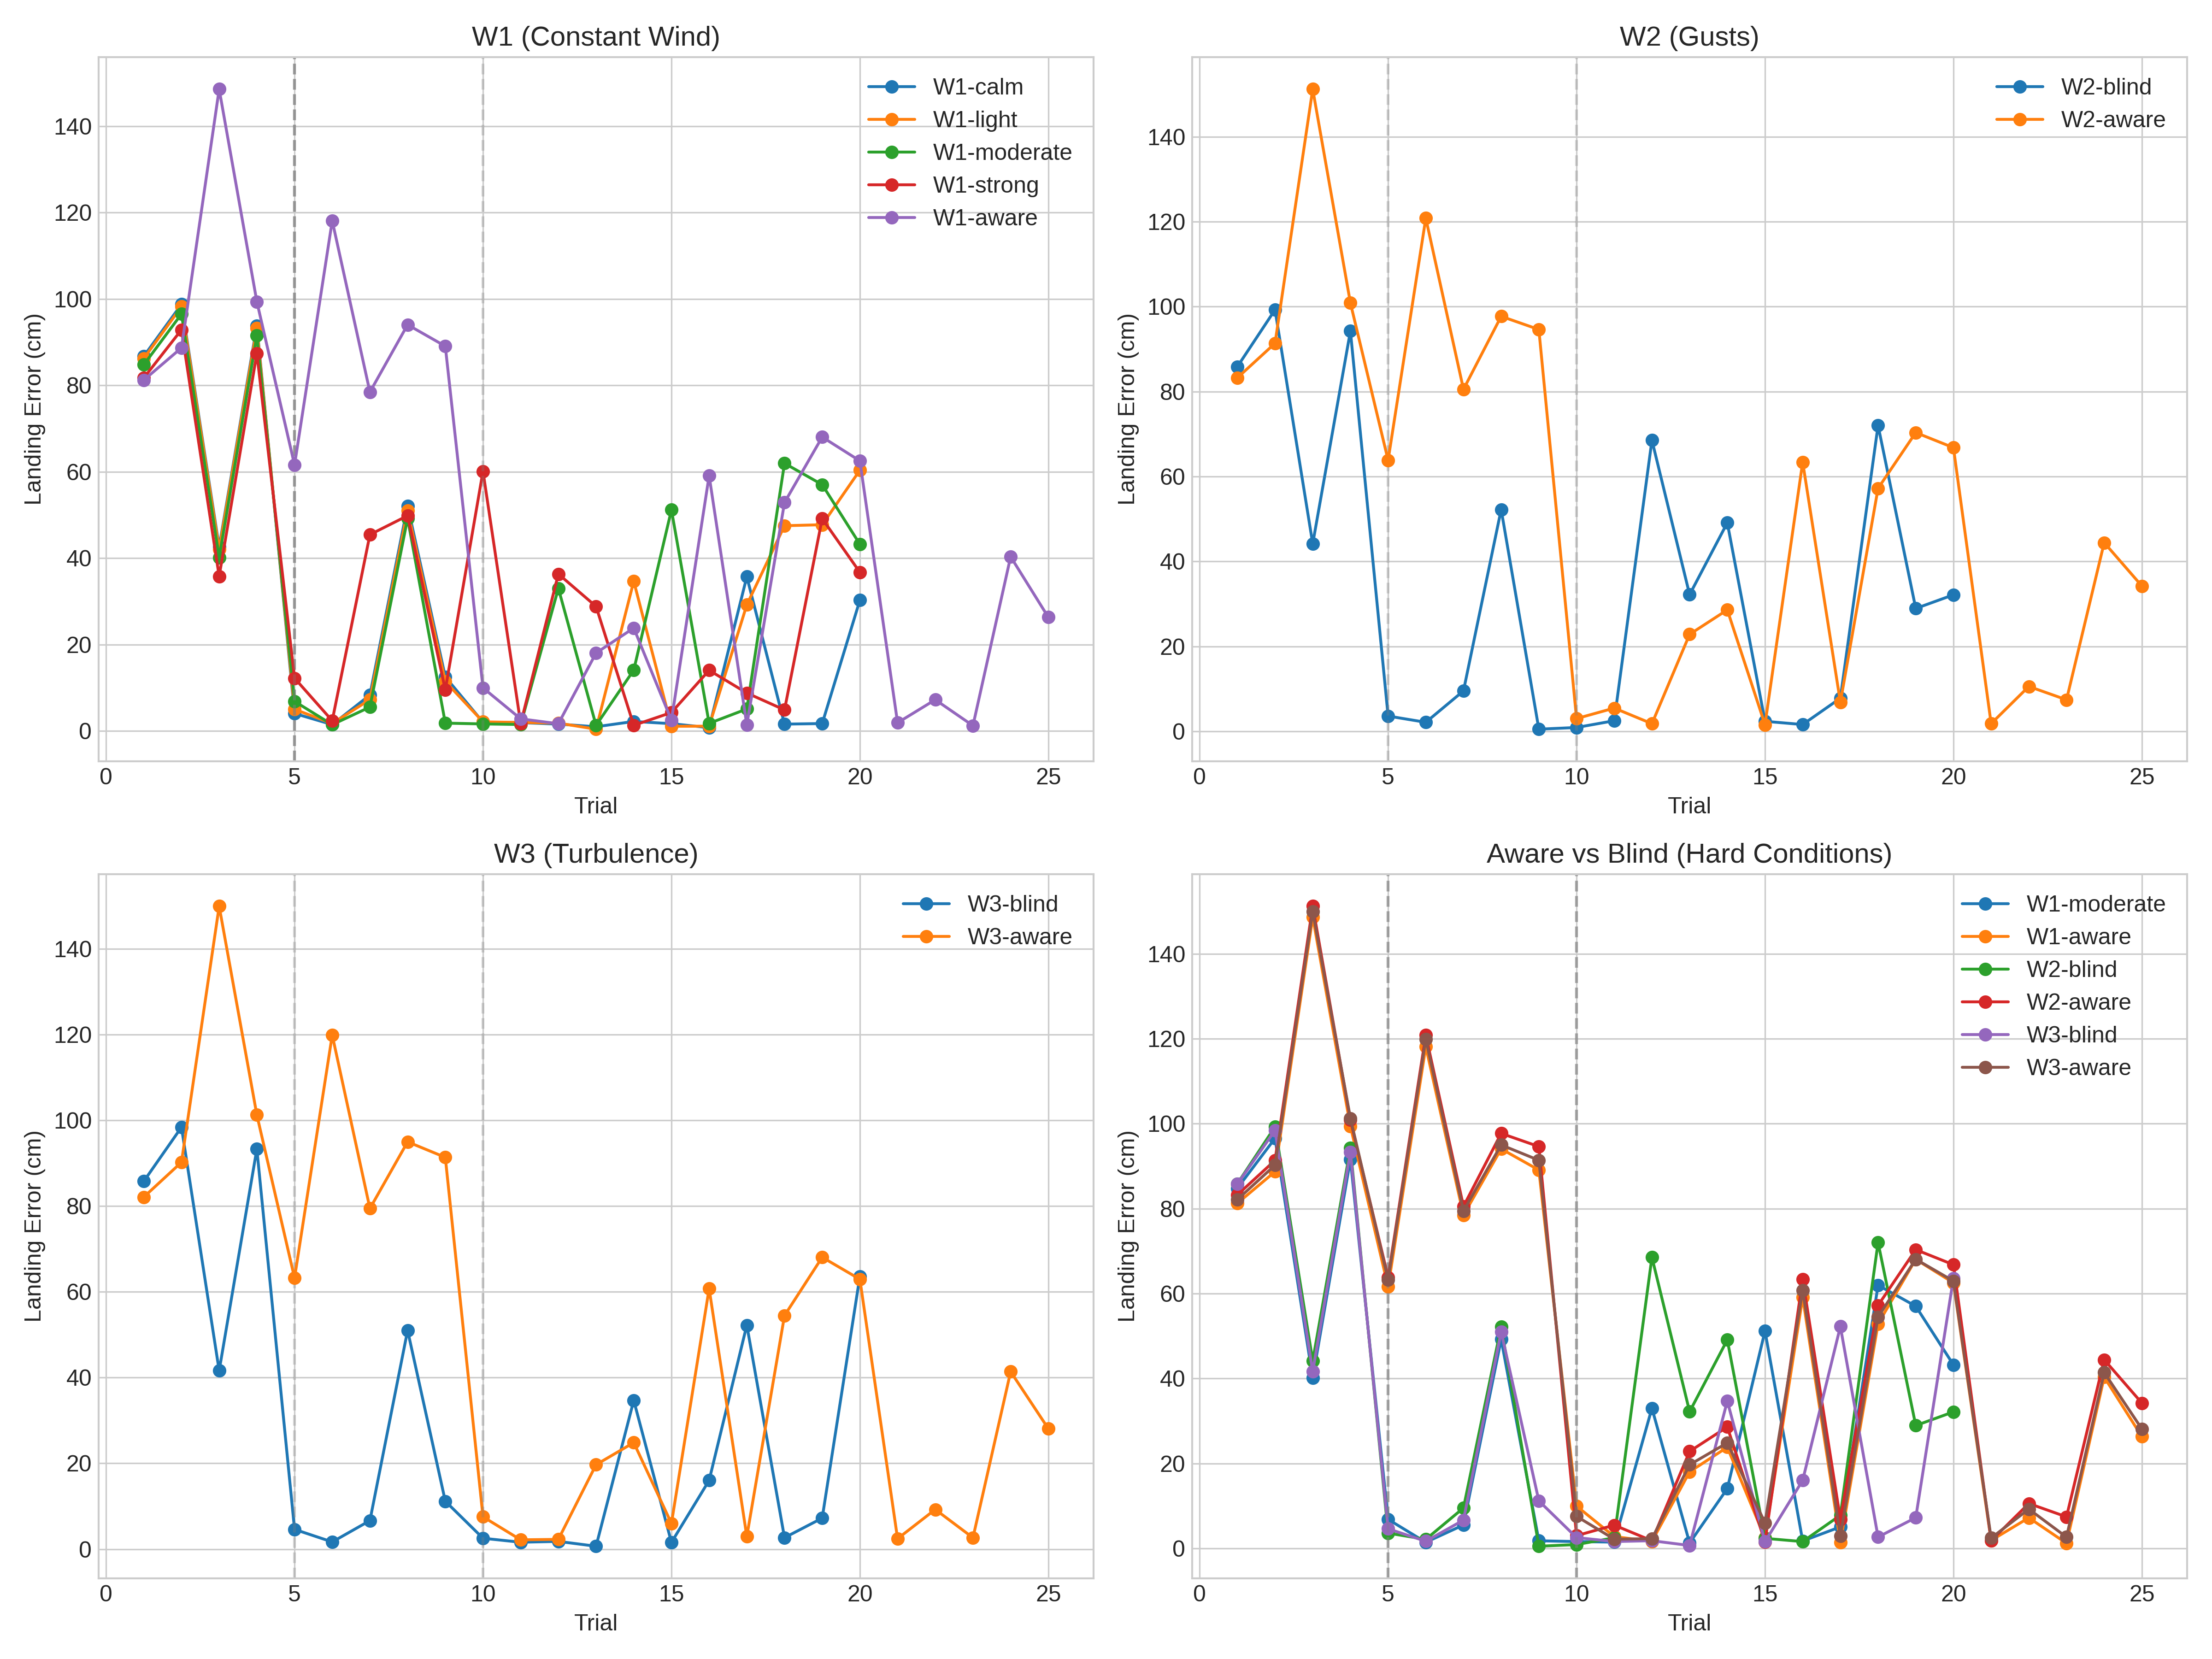
\includegraphics[width=0.85\textwidth]{performance_analysis_plots/learning_curves_error.png}
        \caption{Physical mean error convergence over successive optimization trials.}
    \end{figure}
\end{frame}

\begin{frame}{Performance Analysis: Target Landing Distributions}
    \begin{figure}
        \centering
        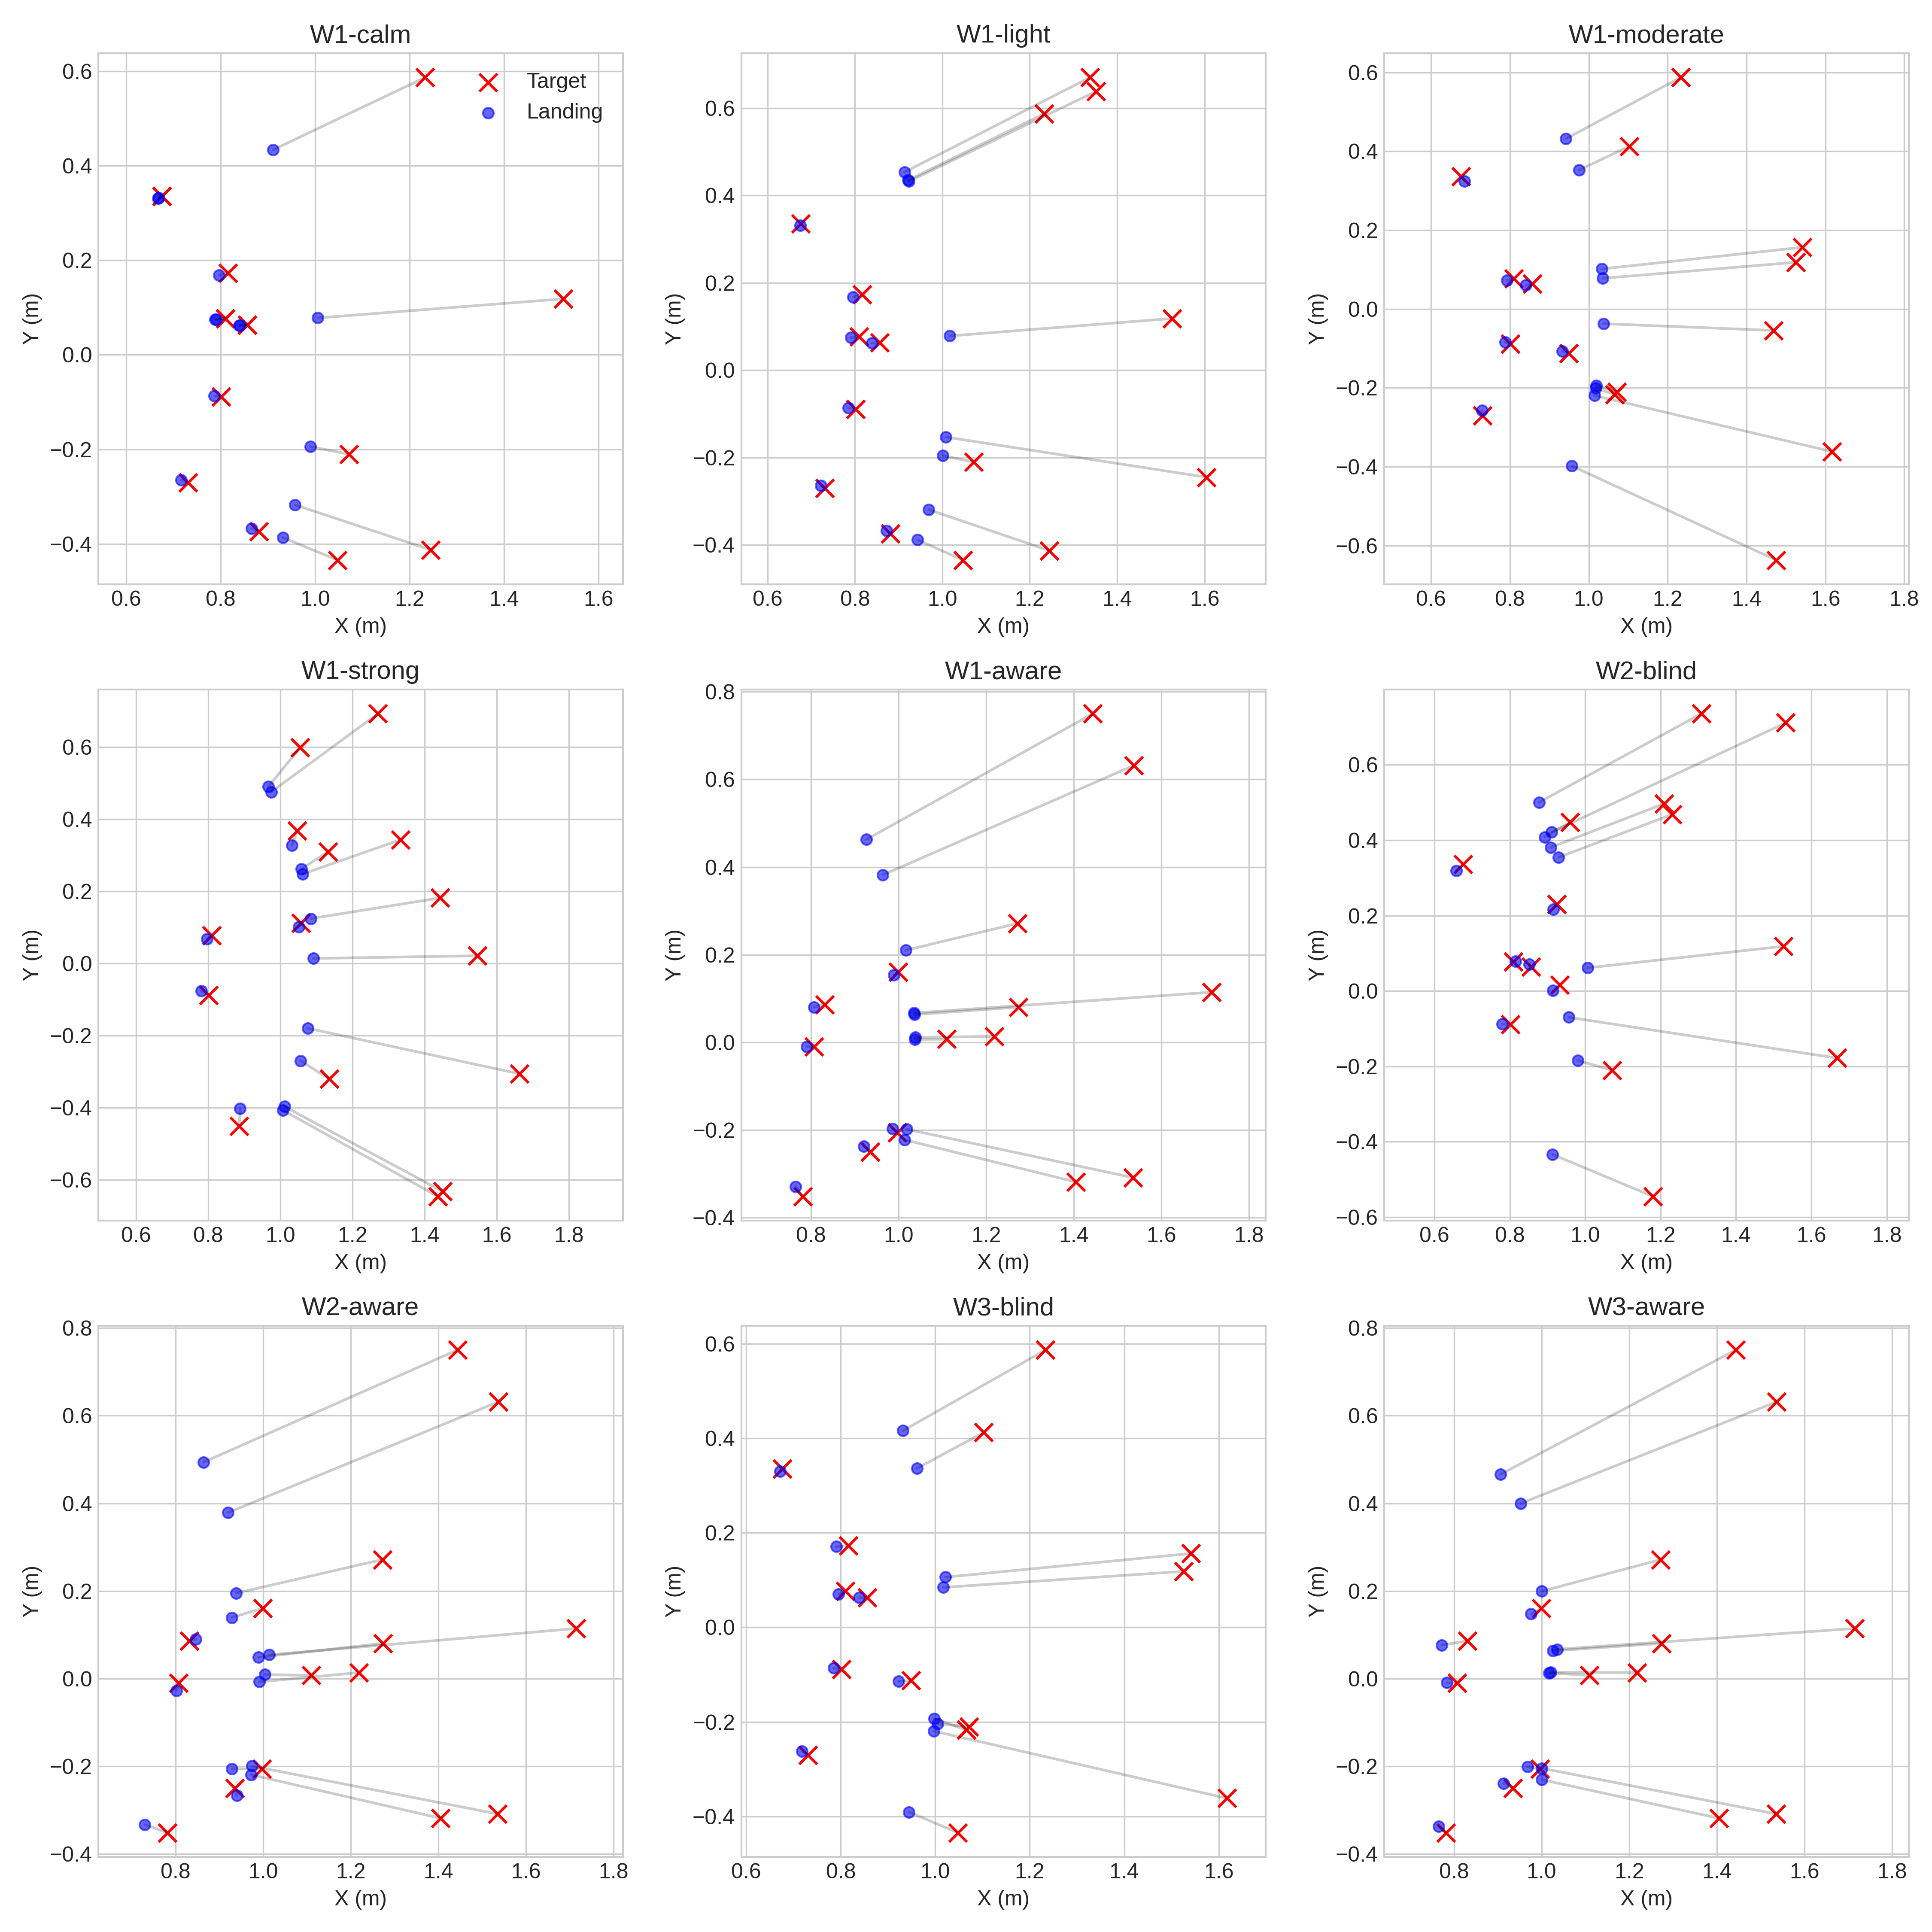
\includegraphics[width=0.75\textwidth]{performance_analysis_plots/scatter_2d_landings.png}
        \caption{2D mapping of actual landing coordinates relative to target positions.}
    \end{figure}
\end{frame}


%%%%%%%%%%%%%%%%%%%%%%%%%%%%%%%%%%%%%%%%%%%%%%%%%%%%%%%%%%%%%
\section{Study 5: Vision Pipeline}

\begin{frame}{OpenCV + YOLO Bin Detection}
    \begin{block}{Problem}
        So far, target coordinates are given numerically. For real deployment, the robot must \textit{detect} the bin visually.
    \end{block}

    \begin{columns}[T]
        \begin{column}{0.48\textwidth}
            \textbf{OpenCV (Geometric)}
            \begin{itemize}
                \item Depth camera on arm base (PyBullet RGB-D)
                \item Segment green bin by HSV threshold $\rightarrow$ contour $\rightarrow$ centroid
                \item Depth back-projection: pixel $(u,v,d) \rightarrow$ world $(x,y)$
                \item Bias correction: camera sees near face of bin $\rightarrow$ shift by $2R/\pi$
            \end{itemize}
        \end{column}
        \begin{column}{0.48\textwidth}
            \textbf{YOLO (Learning-Based)}
            \begin{itemize}
                \item Synthetic dataset: 800 train / 200 val images rendered in PyBullet
                \item YOLOv8n trained on rendered red sphere target
                \item Bounding box centroid + depth $\rightarrow$ 3D target estimate
                \item Robust to occlusion and lighting variation
            \end{itemize}
        \end{column}
    \end{columns}

    \vspace{0.3em}
    Both pipelines feed detected $(x,y)$ into policy $\rightarrow$ throw command. Bin is \textbf{hollow} $\rightarrow$ ball physically enters bin.
    We have also tested the algorithm on different positions of camera.
\end{frame}

%%%%%%%%%%%%%%%%%%%%%%%%%%%%%%%%%%%%%%%%%%%%%%%%%%%%%%%%%%%%

\begin{frame}{Full System Architecture}
\begin{center}
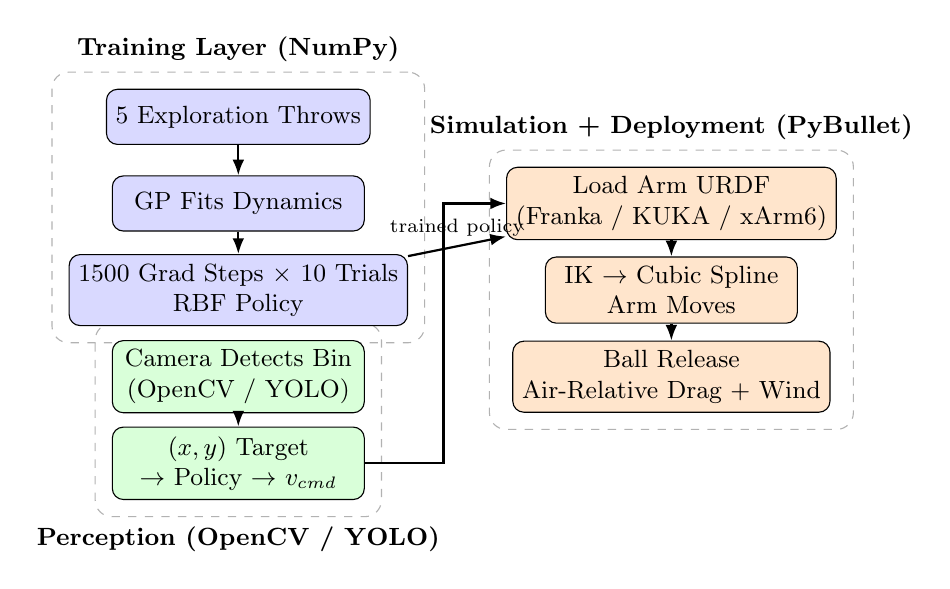
\begin{tikzpicture}[
    box/.style={draw, rounded corners=4pt, minimum width=3.2cm, minimum height=0.7cm,
                font=\small, align=center},
    layer/.style={draw=gray!60, dashed, rounded corners=6pt, inner sep=6pt},
    arr/.style={-{Latex[length=2mm]}, thick},
    font=\small
]
% Training layer
\node[box, fill=blue!15] (exp)  at (0,0)     {5 Exploration Throws};
\node[box, fill=blue!15] (gp)   at (0,-1.1)  {GP Fits Dynamics};
\node[box, fill=blue!15] (opt)  at (0,-2.2)  {1500 Grad Steps $\times$ 10 Trials\\RBF Policy};

% Deployment layer
\node[box, fill=orange!20] (urdf) at (5.5,-1.1) {Load Arm URDF\\(Franka / KUKA / xArm6)};
\node[box, fill=orange!20] (ik)   at (5.5,-2.2) {IK $\rightarrow$ Cubic Spline\\Arm Moves};
\node[box, fill=orange!20] (fly)  at (5.5,-3.3) {Ball Release\\Air-Relative Drag + Wind};

% Perception layer
\node[box, fill=green!15] (cam)  at (0,-3.3)  {Camera Detects Bin\\(OpenCV / YOLO)};
\node[box, fill=green!15] (tgt)  at (0,-4.4)  {$(x,y)$ Target\\$\rightarrow$ Policy $\rightarrow$ $v_\text{cmd}$};

% Arrows training
\draw[arr] (exp) -- (gp);
\draw[arr] (gp) -- (opt);

% Arrow: policy to deployment
\draw[arr] (opt) -- node[above, font=\scriptsize]{trained policy} (urdf);

% Arrows deployment
\draw[arr] (urdf) -- (ik);
\draw[arr] (ik) -- (fly);

% Arrow: perception feeds policy
\draw[arr] (cam) -- (tgt);
\draw[arr] (tgt.east) -- ++(1.0,0) |- (urdf.west);

% Layer backgrounds
\begin{pgfonlayer}{background}
  \node[layer, fit=(exp)(gp)(opt), label=above:{\textbf{Training Layer (NumPy)}}] {};
  \node[layer, fit=(urdf)(ik)(fly), label=above:{\textbf{Simulation + Deployment (PyBullet)}}] {};
  \node[layer, fit=(cam)(tgt), label=below:{\textbf{Perception (OpenCV / YOLO)}}] {};
\end{pgfonlayer}
\end{tikzpicture}
\end{center}
\vspace{0.2em}
\end{frame}

%%%%%%%%%%%%%%%%%%%%%%%%%%%%%%%%%%%%%%%%%%%%%%%%%%%%%%%%%%%%%
\section{Results Summary}

\begin{frame}{Complete Results Summary}
    \begin{center}
    \scriptsize
    \begin{tabular}{lllp{3.8cm}}
        \toprule
        \textbf{Study} & \textbf{Configuration} & \textbf{Hit Rate} & \textbf{Key Insight} \\
        \midrule
        Baseline        & $z=0.5$\,m, Franka, no noise     & \textbf{5/5 (100\%)}      & Cost $0.74\to0.001$ in 5 trials \\
        Elevated        & $z=1.0$\,m, stratified           & \textbf{10/10}            & Pedestal + stratified essential \\
        Elevated        & $z=1.5$\,m, stratified           & \textbf{10/10}            & $\ell_M$, $T$ scaled with height \\
        Elevated        & $z=2.0$\,m, stratified           & \textbf{10/10}            & 10 consecutive hits \\
        Multi-arm       & Franka/KUKA/xArm6               & \textbf{100\% each}       & Arm-agnostic RL validated \\
        Noise           & Slip $\alpha=0.20$, aware        & \textbf{100\% vs 0\%} naive & Infinite relative improvement \\
        Noise           & Salt-pepper $p=0.05$, aware      & \textbf{100\% vs 75\%} naive & Consistent advantage \\
        Wind            & W1 calm, blind                   & 73\%                      & GP learns physics well \\
        Wind            & W3 turbulence, blind             & \textbf{60\% vs 47\%} aware & Implicit beats explicit \\
        Vision          & OpenCV + YOLO                    & End-to-end                & Detect $\rightarrow$ throw in one loop \\
        \bottomrule
    \end{tabular}
    \end{center}
\end{frame}

%%%%%%%%%%%%%%%%%%%%%%%%%%%%%%%%%%%%%%%%%%%%%%%%%%%%%%%%%%%%%
\section{Key Contributions}

\begin{frame}{Key Scientific Contributions}
    \textbf{Three things the paper never stated that are necessary for the algorithm to work:}

    \begin{enumerate}
        \item \textbf{Stratified Exploration} --- random seed can produce zero-coverage exploration; stratified band partitioning guarantees learning regardless of seed
        \vspace{0.3em}
        \item \textbf{RBF Lengthscale Rule} --- $\ell_s \approx 0.15 \times \Delta_\text{range}$; at $\ell_s = 1.0$\,m and range $= 0.35$\,m, policy outputs a constant speed for \textit{all} targets
        \vspace{0.3em}
        \item \textbf{Zero-Mean Noise Invariance (formally proven)} --- symmetric Gaussian noise cannot be compensated by RL; only \textit{biased} noise (slip, timing jitter) is learnable. Paper's gripper delay model is biased, which is why it works on hardware.
    \end{enumerate}

    \vspace{0.5em}
    % \begin{alertblock}{Unexpected Finding}
    %     GP treats constant wind as an \textbf{implicit dynamics bias} --- explicit wind state augmentation \textit{hurts} in low-data regimes due to the curse of dimensionality. 15 trials in 4D policy space $\equiv$ 4 trials in 2D.
    % \end{alertblock}
\end{frame}

%%%%%%%%%%%%%%%%%%%%%%%%%%%%%%%%%%%%%%%%%%%%%%%%%%%%%%%%%%%%%
\section{Future Work}

\begin{frame}{Future Work}
    \begin{itemize}
        \item \textbf{Hardware validation} --- run trained policies on a real robot arm; measure PyBullet-to-real transfer degradation and where the 5--10\% drag discrepancy compounds with real-world effects
        \vspace{0.4em}
        \item \textbf{Wind-robust policy} --- randomise wind per rollout during training so a single policy handles a \textit{distribution} of wind conditions, not one fixed vector
        \vspace{0.4em}
        \item \textbf{End-to-end YOLO deployment} --- vision detection $\rightarrow$ policy $\rightarrow$ throw $\rightarrow$ physical landing in bin, fully in one hardware loop
        \vspace{0.4em}
        \item \textbf{Multi-target sequences} --- policy throws to a sequence of bins without retraining; requires online target switching
        \vspace{0.4em}
        \item \textbf{Adaptive noise estimation} --- estimate slip/jitter parameters \textit{online} via Bayesian Optimisation (paper's approach) rather than requiring them upfront; integrate with the wind-aware pipeline
    \end{itemize}
\end{frame}

%%%%%%%%%%%%%%%%%%%%%%%%%%%%%%%%%%%%%%%%%%%%%%%%%%%%%%%%%%%%%
\begin{frame}[c]
    \centering
    {\Huge \textbf{Thank You!}}\\[1em]
\end{frame}

\end{document}